\chapter{Vận tốc nhóm, nguyên lý loại trừ fermion và biển Dirac}

\section{Vận tốc pha và vận tốc nhóm}

\begin{classroomqa}
\lecturetimestamp{00:00:07}
\audiencequestion{Vận tốc nhóm và vận tốc pha là gì?}
\lecturerresponse{Vận tốc pha bám theo một điểm có pha cố định trong sóng phẳng. Nói chung, nó không mô tả chuyển động của một vật có thể đo được. Vận tốc nhóm bám theo bao sóng của một gói sóng và là vận tốc gắn với hạt, tín hiệu và dòng xác suất.}
\end{classroomqa}

Bắt đầu với một sóng phẳng,
\begin{equation}
\psi(x,t)=e^{i(kx-\omega t)},
\end{equation}
hoặc với dạng thực của nó,
\begin{equation}
\psi(x,t)=\sin(kx-\omega t).
\end{equation}
Một đỉnh sóng, một đáy sóng, hoặc bất kỳ điểm nào khác có pha cố định đều chuyển động sao cho
\begin{equation}
kx-\omega t=\text{constant}.
\end{equation}
Chọn hằng số bằng 0 cho tiện, ta được
\begin{equation}
x=\frac{\omega}{k}t,
\qquad
v_{\mathrm{phase}}=\frac{\omega}{k}.
\end{equation}
Vì \(\omega=2\pi/T\) và \(k=2\pi/\lambda\),
\begin{equation}
v_{\mathrm{phase}}=\frac{\omega}{k}=\frac{\lambda}{T}.
\end{equation}
Đây chính là quãng đường mà một pha cho trước tiến được trong một chu kỳ.

Đối với sóng Schr\"odinger phi tương đối tính, với \(\hbar=1\), năng lượng và xung lượng lần lượt là \(\omega\) và \(k\), nên
\begin{equation}
\omega(k)=\frac{k^2}{2m}.
\end{equation}
Vì vậy vận tốc pha của nó là
\begin{equation}
v_{\mathrm{phase}}=\frac{k}{2m}.
\end{equation}
Tuy nhiên, vận tốc thông thường của một hạt có xung lượng \(k\) là \(k/m\). Sự lệch nhau một hệ số 2 là cảnh báo đầu tiên cho thấy chuyển động của pha của sóng phẳng không phải là chuyển động của hạt.

Còn có một cảnh báo rõ nét hơn nữa. Hãy cộng cùng một hằng số \(C\) vào mọi tần số:
\begin{equation}
\omega(k)\longrightarrow \omega(k)+C.
\end{equation}
Chẳng hạn, hằng số đó có thể biểu diễn một phần đóng góp năng lượng nghỉ chung như \(mc_{\mathrm{light}}^2\), nhưng tên gọi cụ thể của nó không quan trọng. Ở đây \(C\) là một độ dời năng lượng, không phải tốc độ ánh sáng. Vận tốc pha đổi thành
\begin{equation}
v_{\mathrm{phase}}\longrightarrow
\frac{\omega(k)+C}{k}
=v_{\mathrm{phase}}+\frac{C}{k}.
\end{equation}
Thế nhưng, việc cộng cùng một hằng số vào mọi năng lượng không làm thay đổi bất kỳ hiệu năng lượng nào và do đó không làm thay đổi vật lý phi tương đối tính nào.

Có thể thấy điều này trực tiếp trong hàm sóng. Viết một trường Schr\"odinger tổng quát dưới dạng tổng hoặc tích phân các mode,
\begin{equation}
\psi(x,t)=\sum_k a_k e^{ikx}e^{-i\omega(k)t},
\end{equation}
với các hệ số chuẩn hóa được lược bỏ. Sau phép dời,
\begin{align}
\psi(x,t)
&\longrightarrow
\sum_k a_k e^{ikx}e^{-i[\omega(k)+C]t}
\\
&=e^{-iCt}\psi(x,t).
\end{align}
Mỗi mode đều thu được cùng một pha phụ thuộc thời gian. Trường liên hợp thu được pha ngược lại, và do đó
\begin{equation}
\begin{aligned}
\psi^*(x,t)\psi(x,t)
&\longrightarrow
e^{iCt}e^{-iCt}\psi^*(x,t)\psi(x,t)
\\
&=\psi^*(x,t)\psi(x,t).
\end{aligned}
\end{equation}
Sự triệt tiêu tương tự cũng xảy ra trong các giá trị kỳ vọng. Một đại lượng thay đổi khi mốc 0 của năng lượng bị dịch chuyển thì không thể là tốc độ lan truyền vật lý của hạt Schr\"odinger. Vì vậy vận tốc pha phần nào mang tính quy ước.

Một hạt định xứ không được biểu diễn bởi một sóng phẳng vô hạn đơn lẻ mà bởi một gói sóng. Các sóng thành phần giao thoa tăng cường trong vùng của gói và giao thoa triệt tiêu ở bên ngoài. Chuyển động của mẫu hình này đã có thể được tìm ra từ hai sóng lân cận:
\begin{equation}
\psi(x,t)=
\sin(kx-\omega t)+
\sin(k'x-\omega't),
\end{equation}
trong đó \(k'\) gần với \(k\) và \(\omega'=\omega(k')\). Một quỹ tích của giao thoa tăng cường xuất hiện ở nơi các pha của chúng trùng nhau,
\begin{equation}
kx-\omega t=k'x-\omega't.
\end{equation}
Do đó
\begin{equation}
(k-k')x=(\omega-\omega')t,
\end{equation}
và mẫu hình tăng cường chuyển động theo
\begin{equation}
x=\frac{\omega-\omega'}{k-k'}t.
\end{equation}
Lấy giới hạn hai sóng lân cận, ta được
\begin{equation}
x=\frac{d\omega}{dk}t,
\qquad
v_{\mathrm{group}}=\frac{d\omega}{dk}.
\end{equation}
Đây là vận tốc của bao sóng---cụm định xứ được tạo ra bởi sự giao thoa của các sóng thành phần.

Đối với hệ thức tán sắc phi tương đối tính, kể cả độ dời tùy ý,
\begin{equation}
\omega(k)=\frac{k^2}{2m}+C,
\end{equation}
vận tốc nhóm là
\begin{equation}
v_{\mathrm{group}}
=\frac{d}{dk}\left(\frac{k^2}{2m}+C\right)
=\frac{2k}{2m}
=\frac{k}{m}.
\end{equation}
Hằng số cộng thêm đã biến mất, và kết quả chính xác là vận tốc hạt cổ điển.

\begin{classroomqa}
\lecturetimestamp{00:16:35}
\audiencequestion{Hệ số 2 có biến mất trong vận tốc nhóm không?}
\lecturerresponse{Có. Lấy đạo hàm \(k^2\) cho ra \(2k\), triệt tiêu số 2 trong \(2m\). Kết quả là \(k/m\).}
\end{classroomqa}

Do đó, vận tốc nhóm là vận tốc gắn gần nhất với chuyển động hạt cổ điển. Nó cũng là vận tốc thích hợp cho sự lan truyền của một gói sóng và, trong các hoàn cảnh thông thường đang xét ở đây, cho sự lan truyền của tín hiệu. Vận tốc pha không nhất thiết mang một trong hai ý nghĩa đó.

\subsection{Sóng tương đối tính không khối lượng và có khối lượng}

\begin{classroomqa}
\lecturetimestamp{00:17:47}
\audiencequestion{Điều này có liên quan đến những khẳng định rằng ánh sáng có thể truyền nhanh hơn ánh sáng không?}
\lecturerresponse{Không. Những khẳng định đó nêu ra một vấn đề riêng. Một phép tính liên quan quả thật cho thấy một pha có thể chuyển động nhanh hơn ánh sáng trong khi vận tốc nhóm vật lý vẫn dưới tốc độ ánh sáng, nhưng điều đó không mô tả một tín hiệu vượt ánh sáng.}
\end{classroomqa}

\begin{classroomqa}
\lecturetimestamp{00:18:05}
\audiencequestion{Ví dụ liên quan ở đây có phải là trường hợp quen thuộc trong đó vận tốc pha vượt quá tốc độ ánh sáng, trong khi vận tốc nhóm vẫn thấp hơn tốc độ đó không?}
\lecturerresponse{Vâng. Mô thức tương tự cũng xuất hiện đối với một sóng tương đối tính có khối lượng khác không, và điều này suy ra trực tiếp từ hệ thức năng lượng--động lượng tương đối tính.}
\end{classroomqa}

Đặt \(\hbar=c_{\mathrm{light}}=1\). Hệ thức tương đối tính là
\begin{equation}
E=\sqrt{p^2+m^2},
\qquad
\omega(k)=\sqrt{k^2+m^2}.
\end{equation}
Trước hết, hữu ích là xét trường hợp không khối lượng. Khi \(m=0\),
\begin{equation}
\omega=|k|.
\end{equation}
Trên nhánh truyền sang phải \(k>0\), \(\omega=k\), và do đó
\begin{equation}
v_{\mathrm{phase}}=\frac{\omega}{k}=1,
\qquad
v_{\mathrm{group}}=\frac{d\omega}{dk}=1.
\end{equation}
Trên nhánh truyền sang trái, cả hai vận tốc đều mang dấu âm tương ứng. Trong cả hai trường hợp, độ lớn của chúng bằng tốc độ ánh sáng. Vì hệ thức tán sắc là tuyến tính trên mỗi nhánh, mọi thành phần Fourier trên nhánh đó đều chuyển động với cùng một vận tốc.

Đối với một hạt có khối lượng, khi \(k>0\),
\begin{equation}
v_{\mathrm{phase}}
=\frac{\omega}{k}
=\sqrt{\frac{k^2+m^2}{k^2}}>1,
\end{equation}
trong khi
\begin{equation}
v_{\mathrm{group}}
=\frac{d\omega}{dk}
=\frac{k}{\sqrt{k^2+m^2}}<1.
\end{equation}
Với \(k<0\), cả hai vận tốc đều đảo dấu, còn độ lớn của chúng vẫn tuân theo cùng các bất đẳng thức ấy. Vì vậy pha có thể chuyển động nhanh hơn ánh sáng, trong khi gói sóng, hạt, năng lượng và tín hiệu chuyển động chậm hơn ánh sáng. Đối với riêng hệ thức tán sắc này và \(k\neq0\),
\begin{equation}
v_{\mathrm{phase}}v_{\mathrm{group}}=1.
\end{equation}
Quan hệ nghịch đảo đó là một sự ngẫu nhiên của hệ thức tán sắc căn bậc hai, chứ không phải một tính chất tổng quát của sóng.

\begin{figure}
\centering
\includegraphics[width=0.72\textwidth]{lecture_05_figure_03.png}
\caption{Các hệ thức tán sắc phi tương đối tính và tương đối tính, với vận tốc pha \(\omega/k\) và vận tốc nhóm \(d\omega/dk\).}
\lectureframe{00:35:52}
\end{figure}

\begin{classroomqa}
\lecturetimestamp{00:23:41}
\audiencequestion{Hiện tượng tán sắc có gắn với việc tốc độ sóng phụ thuộc vào tần số không?}
\lecturerresponse{Có. Khi \(\omega(k)\) là tuyến tính, mọi thành phần Fourier đều có cùng vận tốc nhóm và một gói sóng có thể giữ nguyên hình dạng. Khi \(\omega(k)\) là phi tuyến, các thành phần khác nhau chuyển động với các vận tốc khác nhau, nên gói sóng bị tán sắc và đổi dạng. Âm thanh tần số thấp xấp xỉ là không tán sắc khi tần số của nó gần như tỉ lệ với số sóng.}
\end{classroomqa}

Vận tốc pha thông thường không mang tín hiệu, năng lượng hay dòng xác suất nào. Giá trị số của nó thậm chí còn có thể thay đổi nếu dịch chuyển mốc 0 của năng lượng. Vận tốc nhóm là chuyển động có ý nghĩa vật lý của một gói sóng đủ hẹp.

\begin{classroomqa}
\lecturetimestamp{00:25:14}
\audiencequestion{Có thể đo vận tốc pha đối với một photon không?}
\lecturerresponse{Trong chân không, photon có tán sắc tuyến tính, nên vận tốc pha và vận tốc nhóm của nó trùng nhau và đều bằng tốc độ ánh sáng. Trong một môi trường vật chất, hệ thức tán sắc thay đổi, và vận tốc pha cùng vận tốc nhóm không nhất thiết trùng nhau.}
\end{classroomqa}

\begin{classroomqa}
\lecturetimestamp{00:25:50}
\audiencequestion{Thảo luận này có bị giới hạn ở các gói sóng không loe rộng theo thời gian không?}
\lecturerresponse{Một gói chỉ giữ không loe rộng khi tất cả các thành phần Fourier của nó có cùng một vận tốc, điều này tương ứng với một hệ thức tán sắc tuyến tính trên khoảng liên quan. Với tán sắc phi tuyến, các thành phần tách xa nhau và gói sóng loe rộng.}
\end{classroomqa}

Các câu hỏi về nón ánh sáng và cấu trúc nhân quả tương đối tính đòi hỏi nhiều hơn sự phân biệt giữa vận tốc pha và vận tốc nhóm, nên được tách riêng khỏi phép tính này.

\section{Đối xứng tịnh tiến và các định luật bảo toàn}

Chính các pha sóng phẳng ấy cho một cách trình bày cô đọng về các định luật bảo toàn. Bắt đầu với bảo toàn năng lượng. Một trường hủy tác dụng lên một hạt tới có năng lượng \(\omega_j\) đóng góp một thừa số thời gian
\begin{equation}
e^{-i\omega_j t},
\end{equation}
trong khi một trường tạo tạo ra một hạt ra có năng lượng \(\omega'_r\) đóng góp
\begin{equation}
e^{+i\omega'_r t}.
\end{equation}
Đối với nhiều hạt tới và hạt ra, tích của chúng là
\begin{equation}
\exp\!\left[
i\left(\sum_r\omega'_r-\sum_j\omega_j\right)t
\right].
\end{equation}
Nếu tương tác có thể xảy ra ở bất kỳ thời điểm nào với cùng một biên độ, thì biên độ bao gồm một tích phân theo thời gian tương tác:
\begin{equation}
\begin{aligned}
&\int_{-\infty}^{\infty}dt\,
\exp\!\left[
i\left(\sum_r\omega'_r-\sum_j\omega_j\right)t
\right]
\\
&\quad =2\pi\,
\delta\!\left(\sum_r\omega'_r-\sum_j\omega_j\right).
\end{aligned}
\end{equation}
Hàm delta buộc tổng năng lượng ra phải bằng tổng năng lượng tới. Cùng một biên độ ở mọi thời điểm tương tác khả dĩ là bất biến tịnh tiến theo thời gian, và nó sinh ra bảo toàn năng lượng.

Tịnh tiến trong không gian cho bảo toàn xung lượng bằng cùng cơ chế ấy. Xét một phân rã vật lý một thành hai, trong đó một hạt tới có xung lượng \(k\) biến mất và hai hạt có xung lượng \(k'_1\) và \(k'_2\) xuất hiện. Một tương tác địa phương tại vị trí \(x\) chứa một trường hủy và hai trường tạo,
\begin{equation}
\mathcal{O}(x)=\psi^\dagger(x)\psi^\dagger(x)\psi(x).
\end{equation}
Bỏ qua sự phụ thuộc theo thời gian và các hệ số chuẩn hóa, các thừa số mode liên quan là
\begin{align}
\psi(x)&\supset a_k e^{ikx},
\\
\psi^\dagger(x)&\supset a_{k'_1}^\dagger e^{-ik'_1x},
\qquad
\psi^\dagger(x)\supset a_{k'_2}^\dagger e^{-ik'_2x}.
\end{align}
Trong phần tử ma trận
\begin{equation}
\langle k'_1,k'_2|\mathcal{O}(x)|k\rangle,
\end{equation}
toán tử hủy loại bỏ hạt tới và hai toán tử tạo cung cấp các hạt ra. Sau khi thực hiện các tác dụng toán tử đó, thừa số phụ thuộc vị trí còn lại là
\begin{equation}
e^{-ik'_1x}e^{-ik'_2x}e^{ikx}
=e^{i(k-k'_1-k'_2)x}.
\end{equation}
Vì không có vị trí nào được ưu tiên, ta tích phân trên mọi vị trí phân rã khả dĩ:
\begin{equation}
\int_{-\infty}^{\infty}dx\,
e^{i(k-k'_1-k'_2)x}
=2\pi\delta(k-k'_1-k'_2).
\end{equation}
Vì thế biên độ còn lại tuân theo
\begin{equation}
k=k'_1+k'_2.
\end{equation}
Trong ba chiều, cùng phép tính ấy dùng \(d^3x\), các vectơ xung lượng in đậm và một hàm delta ba chiều. Không điều gì trong lập luận này phụ thuộc vào việc chỉ có một hạt tới hay hai hạt ra. Với số hạt bất kỳ, tích phân trên vị trí tương tác chung cho ra
\begin{equation}
\delta^{(3)}\!\left(
\sum_j\mathbf{k}_j-\sum_r\mathbf{k}'_r
\right).
\end{equation}
Cùng một biên độ ở mọi vị trí là bất biến tịnh tiến trong không gian, và nó cho bảo toàn xung lượng đúng như cùng một biên độ ở mọi thời điểm cho bảo toàn năng lượng.

Ví dụ thứ ba là một phép quay pha toàn cục,
\begin{equation}
\psi\longrightarrow e^{i\lambda}\psi,
\qquad
\psi^\dagger\longrightarrow e^{-i\lambda}\psi^\dagger.
\end{equation}
Một biên độ tương tác là bất biến khi các pha do những trường hủy và tạo của nó đóng góp triệt tiêu lẫn nhau. Đối với một trường mang điện tích điện, sự bằng nhau giữa điện tích bị lấy đi khỏi trạng thái đầu và được hoàn lại vào trạng thái cuối chính là bảo toàn điện tích. Như vậy, các phép tịnh tiến theo thời gian, các phép tịnh tiến trong không gian và các phép quay pha toàn cục minh họa cách các trường tạo và hủy hạt mã hóa sự bảo toàn năng lượng, xung lượng và điện tích.

\begin{classroomqa}
\lecturetimestamp{00:37:52}
\audiencequestion{Tích phân theo không gian có nghĩa là tích phân trên cả ba chiều không gian phải không?}
\lecturerresponse{Đúng. Ba phép tích phân tạo ra một hàm delta cho ba thành phần xung lượng, nên cả ba thành phần của tổng xung lượng đều được bảo toàn.}
\end{classroomqa}

\begin{classroomqa}
\lecturetimestamp{00:38:03}
\audiencequestion{Mô hình này có xác định các xác suất tương đối cho những cách khác nhau để phân chia xung lượng được bảo toàn không?}
\lecturerresponse{Không. Biểu thức đơn giản này áp đặt tổng các xung lượng ra nhưng ngoài ra không thiên về cách chúng được chia. Các xác suất tương đối đòi hỏi thêm thông tin động lực học.}
\end{classroomqa}

\begin{classroomqa}
\lecturetimestamp{00:39:04}
\audiencequestion{Vì sao một tổng các toán tử hủy lại rút gọn còn hạng khớp với xung lượng đang bị chiếm?}
\lecturerresponse{Một toán tử hủy tác dụng lên một mode trống cho vectơ 0. Nếu trạng thái chỉ chứa một hạt ở mode \(k_0\), thì mọi hạng trừ hạng có \(k=k_0\) đều triệt tiêu.}
\end{classroomqa}

Ví dụ,
\begin{equation}
\sum_k a_k e^{ikx}|1_{k_0}\rangle
=e^{ik_0x}|0\rangle,
\end{equation}
nếu bỏ qua chuẩn hóa: mọi toán tử hủy ứng với các mode trống đều cho vectơ 0.

\section{Sự tăng cường boson và nguyên lý loại trừ fermion}

Boson cho phép bất kỳ số chiếm không âm nào trong một trạng thái một hạt, và đại số của toán tử tạo của chúng thực sự ưu tiên một trạng thái đã bị chiếm sẵn. Đối với một mode boson, quy ước trạng thái số đã chuẩn hóa viết sự tăng cường theo số chiếm dưới dạng\footnote{Bài giảng nêu sự tăng cường theo số chiếm dưới căn bậc hai; phương trình có chỉ số này là dạng chuẩn của nó trong cơ sở trạng thái số.}
\begin{equation}
a^\dagger|n\rangle=\sqrt{n+1}\,|n+1\rangle.
\end{equation}
Giả sử một nguyên tử kích thích có thể phát ra một photon vào nhiều mode có thể có. Khi không có các photon khác, các hướng và động lượng khác nhau xuất hiện theo phân bố xác suất thông thường của chúng. Nếu một mode cụ thể đã chứa nhiều photon---tất cả đều có cùng động lượng, năng lượng và tần số---thì sự phát xạ vào mode đó được tăng cường bởi hệ số theo số chiếm dưới căn bậc hai tương ứng. Nguyên tử sẽ ưu tiên thêm photon của nó vào trạng thái đã có hạt chiếm. Đó là phát xạ kích thích và là một biểu hiện cụ thể của sự tụ tập boson.

Fermion hành xử theo cách ngược lại. Hai fermion đồng nhất không thể chiếm cùng một trạng thái lượng tử. Nguyên lý loại trừ trước hết xuất hiện trong vật lý nguyên tử, nơi hai electron trong một nguyên tử không thể có các số lượng tử giống hệt nhau, nhưng nó không bị giới hạn trong các nguyên tử: các fermion đồng nhất không thể cùng chia sẻ một trạng thái một hạt đầy đủ ở bất cứ đâu.

Khai triển trường ban đầu trông hệt như khai triển boson. Trong một hộp hữu hạn ta có thể viết
\begin{equation}
\psi(x)=\sum_k A_k e^{ikx},
\qquad
\psi^\dagger(x)=\sum_k A_k^\dagger e^{-ikx}.
\end{equation}
Đối với động lượng liên tục, các tổng trở thành các tích phân. Dấu ngược lại trong pha không gian liên hợp suy ra từ phép liên hợp Hermite. Phần này của phép xây dựng là phi tương đối tính; fermion tương đối tính chỉ được đưa vào ở phần cuối.

Trạng thái của trường vẫn được ghi lại bằng một số chiếm cho mỗi mode, nhưng giờ mỗi số chỉ có thể là 0 hoặc 1:
\begin{equation}
|n_{k_1},n_{k_2},\ldots\rangle,
\qquad n_k\in\{0,1\}.
\end{equation}
Không có thêm kiểu hạt tương đối tính nào mà, chẳng hạn, mỗi trạng thái chứa tối đa 3 hạt hoặc ít nhất 7 hạt. Việc xác lập rằng thống kê boson và fermion là những khả năng duy nhất đòi hỏi cơ học lượng tử cùng với thuyết tương đối hẹp và vượt ra ngoài thảo luận hiện tại. Ở đây, nhiệm vụ là mô tả khả năng fermion và các hệ quả của nó.

\subsection{Một trạng thái fermion}

Hãy tập trung vào một trạng thái một hạt duy nhất. Nó hoặc là rỗng, \(|0\rangle\), hoặc bị chiếm, \(|1\rangle\). Toán tử tạo và hủy tác dụng như
\begin{align}
A^\dagger|0\rangle&=|1\rangle,
&
A^\dagger|1\rangle&=0,
\\
A|0\rangle&=0,
&
A|1\rangle&=|0\rangle.
\end{align}
Số 0 không kèm ký hiệu ở vế phải là vectơ không, không phải trạng thái rỗng \(|0\rangle\). Việc cố thêm fermion thứ hai không trả về chân không; nó hoàn toàn không cho ra trạng thái vật lý nào cả.

\begin{classroomqa}
\lecturetimestamp{00:46:25}
\audiencequestion{Các toán tử tạo và hủy fermion vẫn là các toán tử tuyến tính chứ?}
\lecturerresponse{Có. Các toán tử trong cơ học lượng tử là các toán tử tuyến tính, bao gồm cả các toán tử tạo và hủy fermion.}
\end{classroomqa}

\begin{classroomqa}
\lecturetimestamp{00:47:34}
\audiencequestion{Số 0 có nghĩa là trạng thái rỗng, hay có nghĩa là phép tác động được thử không thể tạo ra một trạng thái?}
\lecturerresponse{Nó có nghĩa là vectơ không, không phải trạng thái rỗng. Một trạng thái chân không hay trạng thái cơ bản thực sự có hàm sóng khác không; hàm đồng nhất bằng 0 có chuẩn bằng 0 và không phải là một trạng thái vật lý.}
\end{classroomqa}

Dao động tử điều hòa làm cho sự phân biệt này trở nên cụ thể. Trạng thái cơ bản của nó, tức trạng thái không có kích thích dao động tử, có một hàm sóng Gauss chẳng hạn như
\begin{equation}
\phi_0(q)\propto e^{-\alpha q^2},
\qquad \alpha>0.
\end{equation}
Đây là một trạng thái hoàn toàn tốt và chuẩn hóa được. Ngược lại,
\begin{equation}
\phi(q)\equiv0
\end{equation}
là vectơ không: nó không có biên độ xác suất ở đâu cả và không phải là một trạng thái. Vì vậy \(A^\dagger|1\rangle=0\) nói rằng phép tạo thứ hai được thử tạo ra vectơ không.

\begin{classroomqa}
\lecturetimestamp{00:48:42}
\audiencequestion{Các toán tử fermion có nên dùng ký hiệu khác với các toán tử boson không?}
\lecturerresponse{Có. Rõ ràng hơn nếu dành \(a\) và \(a^\dagger\) cho các mode boson và dùng \(c\) và \(c^\dagger\) cho các mode fermion. Cả hai quy ước đều xuất hiện trong tài liệu, nhưng dùng các chữ khác nhau giúp giữ hai đại số tách biệt.}
\end{classroomqa}

Theo ký hiệu đó, các quy tắc cho một mode duy nhất là
\begin{align}
c^\dagger|0\rangle&=|1\rangle,
&c^\dagger|1\rangle&=0,
\\
c|0\rangle&=0,
&c|1\rangle&=|0\rangle.
\end{align}
Bây giờ hãy tính hai tích có thể có trên cả hai trạng thái cơ sở. Trên trạng thái rỗng,
\begin{align}
c^\dagger c|0\rangle&=0,
&
cc^\dagger|0\rangle&=|0\rangle.
\end{align}
Trên trạng thái bị chiếm,
\begin{align}
c^\dagger c|1\rangle&=|1\rangle,
&
cc^\dagger|1\rangle&=0.
\end{align}
Tổng của chúng trả lại đúng trạng thái mà nó tác dụng lên:
\begin{align}
(c^\dagger c+cc^\dagger)|0\rangle&=|0\rangle,
\\
(c^\dagger c+cc^\dagger)|1\rangle&=|1\rangle.
\end{align}
Vì \(|0\rangle\) và \(|1\rangle\) sinh ra không gian trạng thái của một mode,
\begin{equation}
c^\dagger c+cc^\dagger=1.
\end{equation}
Tổ hợp với dấu cộng là phản giao hoán tử,
\begin{equation}
\{A,B\}=AB+BA,
\end{equation}
nên hệ thức fermion là
\begin{equation}
\{c,c^\dagger\}=1.
\end{equation}
Đó là phép tương tự fermion của giao hoán tử boson
\begin{equation}
[a,a^\dagger]=aa^\dagger-a^\dagger a=1.
\end{equation}

Hai phép tạo trong cùng một trạng thái fermion luôn cho không. Nếu trạng thái còn trống, phép tạo thứ nhất lấp đầy nó và phép tạo thứ hai không thực hiện được; nếu nó đã bị chiếm, thì ngay phép tạo thứ nhất đã không thực hiện được. Tương tự, hai phép hủy cũng luôn cho không. Vì vậy
\begin{equation}
\{c^\dagger,c^\dagger\}=2(c^\dagger)^2=0,
\qquad
\{c,c\}=2c^2=0.
\end{equation}

\begin{classroomqa}
\lecturetimestamp{00:56:45}
\audiencequestion{Số 0 trong hệ thức bình phương của toán tử hủy có phải là vectơ không không?}
\lecturerresponse{Phương trình phát biểu rằng \(c^2\) là toán tử không. Đó là một toán tử biến mọi vectơ trạng thái thành vectơ không. Toán tử không và vectơ không là những đối tượng toán học khác nhau, mặc dù đối tượng thứ nhất luôn cho ra đối tượng thứ hai.}
\end{classroomqa}

Đối với nhiều mode động lượng rời rạc, đại số đầy đủ là
\begin{align}
\{c_k,c_{k'}^\dagger\}&=\delta_{kk'},
\\
\{c_k,c_{k'}\}&=0,
\\
\{c_k^\dagger,c_{k'}^\dagger\}&=0.
\end{align}
Delta Kronecker bằng một khi \(k=k'\) và bằng không trong các trường hợp khác. Đối với động lượng liên tục, với chuẩn hóa thích hợp, nó được thay bằng hàm delta Dirac. Các phản giao hoán tử giữa những toán tử cùng loại đều bằng không với mọi cặp mode, không chỉ khi các nhãn của chúng trùng nhau.

\subsection{Nguyên lý loại trừ trong không gian vị trí}

Đại số được gắn nhãn bởi động lượng trước hết nói rằng hai fermion đồng nhất cùng loại không thể chiếm cùng một mode động lượng. Nó còn nói được nhiều hơn. Một hạt định xứ tại vị trí \(x\) được tạo bởi
\begin{equation}
\psi^\dagger(x)=\sum_k c_k^\dagger e^{-ikx},
\end{equation}
tới một hệ số chuẩn hóa. Tại gốc tọa độ, việc thử tạo hai hạt cho
\begin{align}
\psi^\dagger(0)\psi^\dagger(0)|\Omega\rangle
&=\sum_{k,k'}c_k^\dagger c_{k'}^\dagger|\Omega\rangle.
\end{align}
Các nhãn \(k\) và \(k'\) là các biến tổng giả. Hoán đổi chúng không làm thay đổi tổng kép, vì vậy có thể lấy trung bình nó với dạng đã đổi nhãn của nó:
\begin{align}
\sum_{k,k'}c_k^\dagger c_{k'}^\dagger|\Omega\rangle
&=\frac12\sum_{k,k'}
\left(c_k^\dagger c_{k'}^\dagger
+c_{k'}^\dagger c_k^\dagger\right)|\Omega\rangle
\\
&=\frac12\sum_{k,k'}
\{c_k^\dagger,c_{k'}^\dagger\}|\Omega\rangle
=0.
\end{align}

\begin{classroomqa}
\lecturetimestamp{01:02:26}
\audiencequestion{Chỉ các hạng có động lượng khác nhau mới triệt tiêu trong tổng trạng thái vị trí hai hạt thôi sao?}
\lecturerresponse{Không. Việc đổi nhãn các chỉ số giả biến toàn bộ tổng kép thành một nửa của phản giao hoán tử của hai toán tử tạo. Phản giao hoán tử đó triệt tiêu với mọi cặp động lượng, nên toàn bộ tổng bằng không.}
\end{classroomqa}

Phép tính cho thấy nguyên lý loại trừ không phải là điều riêng có của các trạng thái riêng động lượng. Các fermion đồng nhất cũng không thể chiếm cùng một trạng thái vị trí. Tổng quát hơn, chúng không thể chiếm bất kỳ trạng thái một hạt đồng nhất nào.

\subsection{Thế nào được coi là cùng một trạng thái?}

\begin{classroomqa}
\lecturetimestamp{01:04:30}
\audiencequestion{Hai electron ở rất xa nhau có thể có cùng động lượng không?}
\lecturerresponse{Nguyên lý loại trừ liên quan đến trạng thái một hạt đầy đủ. Hai electron có thể có cùng một trị riêng động lượng chính xác khi chúng khác nhau ở một nhãn giao hoán khác, chẳng hạn spin. Các electron tách biệt trong không gian thì thay vào đó là các gói định xứ chứ không phải các trạng thái riêng động lượng chính xác; các động lượng trung bình của chúng có thể gần như bằng nhau trong khi các hàm sóng không gian vẫn khác nhau. Điều bị cấm là sự trùng nhau của các trạng thái đầy đủ.}
\end{classroomqa}

Spin vẫn chưa được trình bày, nhưng nó cung cấp một nhãn bổ sung quen thuộc. Hai electron có thể cùng chia sẻ một giá trị động lượng khi các trạng thái spin của chúng khác nhau. Khi mọi nhãn liên quan đều đã được tính đến, không hai fermion đồng nhất nào được phép cùng chia sẻ cùng một trạng thái đầy đủ.

\begin{classroomqa}
\lecturetimestamp{01:05:25}
\audiencequestion{Các electron trong hai nguyên tử hydro tách biệt có thể có cùng động lượng hoặc cùng trạng thái nguyên tử không?}
\lecturerresponse{Một electron liên kết trong nguyên tử không phải là trạng thái riêng động lượng. Hàm sóng obitan của nó được định tâm trên nguyên tử đó. Hai nguyên tử tách biệt có thể mỗi nguyên tử đều có một electron ở cái được gọi là trạng thái cơ bản nguyên tử, nhưng một obitan được định tâm trên nguyên tử thứ nhất còn obitan kia trên nguyên tử thứ hai, nên chúng là các trạng thái một hạt khác nhau.}
\end{classroomqa}

\begin{classroomqa}
\lecturetimestamp{01:06:33}
\audiencequestion{Có thể dùng từ tổng quát hơn là hệ để thay cho trạng thái không?}
\lecturerresponse{Không. Một hệ là một tập hợp các bậc tự do; một trạng thái chỉ rõ một cấu hình lượng tử cụ thể của hệ đó. Một electron là một hệ, còn hàm sóng obitan và spin của nó mô tả một trạng thái của hệ ấy.}
\end{classroomqa}

\begin{figure}
\centering
\includegraphics[width=0.74\textwidth]{lecture_05_figure_04.png}
\caption{Các hàm sóng một hạt định xứ và trạng thái với hai toán tử tạo dùng để kiểm tra nguyên lý loại trừ fermion.}
\lectureframe{01:07:21}
\end{figure}

\begin{classroomqa}
\lecturetimestamp{01:07:22}
\audiencequestion{Trong chùm electron của ống tia catốt, có phải không có hai electron nào ở cùng một trạng thái không?}
\lecturerresponse{Có. Các electron chiếm các gói sóng khác nhau, tách biệt về vị trí hoặc được phân biệt theo cách khác trong toàn bộ trạng thái của chúng. Điều này tương phản với photon, vốn có thể cùng chiếm một mode sóng phẳng và tạo nên một chùm kết hợp.}
\end{classroomqa}

Có thể hình dung một chùm electron như một gói định xứ này nối tiếp một gói khác. Các gói ấy không nhất thiết phải là các trạng thái vị trí chính xác hay các trạng thái động lượng chính xác; chỉ cần các hàm sóng của chúng khác nhau là đủ. Ngược lại, một chùm photon có thể có nhiều photon ở chính xác cùng một trạng thái sóng phẳng.

\begin{classroomqa}
\lecturetimestamp{01:08:14}
\audiencequestion{Hai electron có thể ở cùng một vị trí nhưng có các động lượng khác nhau không?}
\lecturerresponse{Vị trí chính xác và động lượng chính xác là các nhãn không tương thích vì các toán tử tương ứng không giao hoán. Không thể chỉ định một trạng thái một hạt bằng vị trí và động lượng đồng thời đều sắc nét. Spin có thể đi kèm với một nhãn vị trí hoặc động lượng vì spin giao hoán với các đại lượng quan sát đó trong bối cảnh phi tương đối tính này.}
\end{classroomqa}

\begin{classroomqa}
\lecturetimestamp{01:08:51}
\audiencequestion{Các electron liên kết ở những nơi tách biệt có xấp xỉ ở các trạng thái vị trí không?}
\lecturerresponse{Chúng không phải là các trạng thái riêng vị trí chính xác, vì mỗi obitan có độ trải không gian hữu hạn, nhưng mỗi cái được định xứ xấp xỉ gần nguyên tử riêng của nó. Sự định xứ đó đủ để làm cho hai hàm sóng obitan là hai trạng thái khác nhau.}
\end{classroomqa}

\begin{classroomqa}
\lecturetimestamp{01:09:31}
\audiencequestion{Định nghĩa của một trạng thái lượng tử là gì?}
\lecturerresponse{Một trạng thái là đối tượng tương tự lượng tử của cấu hình của một hệ. Nó chứa thông tin cần thiết để gán xác suất cho các phép đo có thể xảy ra. Đối với một electron, trạng thái được biểu diễn bởi một hàm sóng, cùng với mọi nhãn nội tại như spin.}
\end{classroomqa}

\begin{classroomqa}
\lecturetimestamp{01:10:32}
\audiencequestion{Các electron được định xứ ở những nơi rất xa nhau có thể ở cùng một trạng thái hoặc có cùng động lượng không?}
\lecturerresponse{Chúng không thể là cùng một trạng thái vì sự định xứ của chúng khác nhau: một electron ở đây và một electron trong thiên hà Andromeda, hoặc một ở Nevada và một ở Connecticut, có các hàm sóng khác nhau. Chúng có thể có các động lượng gần như bằng nhau. Nếu làm một trong hai động lượng trở nên sắc nét vô hạn, hàm sóng tương ứng sẽ trải ra trong không gian và phá hủy sự định xứ vốn phân biệt các trạng thái.}
\end{classroomqa}

Dạng theo độ lệch chuẩn của hệ thức bất định vị trí--động lượng là\footnote{Bài giảng nêu phát biểu định tính về tích bất định; hệ số \(\hbar/2\) được bổ sung theo quy ước độ lệch chuẩn.}
\begin{equation}
\Delta x\,\Delta p\geq\frac{\hbar}{2}.
\end{equation}
Một gói có thể được định xứ ở Nevada và có phân bố động lượng khá hẹp, trong khi một gói khác ở Connecticut có phân bố gần như giống hệt. Chúng vẫn là các trạng thái khác nhau vì các hàm sóng không gian của chúng khác nhau. Trong giới hạn trạng thái riêng động lượng chính xác, không gói nào còn định xứ ở một trong hai nơi đó nữa.

Các toán tử fermion được dùng trong các phản ứng theo cùng cách như các toán tử boson. Một toán tử hủy electron loại bỏ một electron đi vào, một toán tử tạo electron cung cấp một electron đi ra, và các thừa số này có thể được nhân với các toán tử tạo hoặc hủy photon. Photon là boson, còn electron là fermion. Tích của các toán tử ấy cung cấp sự ghi nhận đại số cho các phản ứng có electron đi vào và đi ra cùng với các photon được phát ra hoặc hấp thụ.

\begin{classroomqa}
\lecturetimestamp{01:13:36}
\audiencequestion{Nguyên lý loại trừ Pauli được truyền đi một cách cục bộ, hay được thực thi trên phạm vi toàn cục khi hai quá trình tạo hạt tách biệt nhau trong không gian?}
\lecturerresponse{Nếu biết một hạt ở Nevada và hạt kia ở Connecticut, thì chúng không ở cùng một trạng thái.}
\end{classroomqa}

\editorialnote{Không khôi phục được một đoạn ngắn trong phần trả lời cho câu hỏi này. Sự phân biệt giữa các trạng thái một hạt định xứ và các chồng chập Nevada--Connecticut là chắc chắn.}

Khi vị trí của chúng không xác định, nguyên lý loại trừ xét xem các hàm sóng một hạt đầy đủ có trùng nhau hay không. Các chồng chập Nevada--Connecticut làm cho sự phân biệt đó trở nên tường minh.

Gọi \(|N\rangle\) và \(|C\rangle\) là các trạng thái trực chuẩn định xứ ở Nevada và Connecticut. Khi đó
\begin{equation}
|+\rangle=\frac{|N\rangle+|C\rangle}{\sqrt2},
\qquad
|-\rangle=\frac{|N\rangle-|C\rangle}{\sqrt2}.
\end{equation}
Trạng thái \(|+\rangle\) cho xác suất như nhau để tìm thấy electron trong đó ở Nevada hoặc Connecticut. Trạng thái \(|-\rangle\) cho cùng các xác suất vị trí ấy nhưng khác bởi một pha tương đối. Hai trạng thái này trực giao:
\begin{equation}
\langle+|-\rangle=0.
\end{equation}
Hai electron không thể đồng thời cùng chiếm \(|+\rangle\), và cũng không thể đồng thời cùng chiếm \(|-\rangle\), nhưng nguyên lý loại trừ không ngăn cản một electron ở mỗi trạng thái.

\begin{classroomqa}
\lecturetimestamp{01:16:25}
\audiencequestion{Có thể để một electron chiếm chồng chập cộng Nevada--Connecticut và một electron khác chiếm chồng chập trừ hay không?}
\lecturerresponse{Có. Hai tổ hợp cộng và trừ là trực giao và vì thế là hai trạng thái một hạt khác nhau.}
\end{classroomqa}

\begin{classroomqa}
\lecturetimestamp{01:16:39}
\audiencequestion{Ví dụ về các trạng thái tách biệt có đòi hỏi một khái niệm về tính đồng thời hay không?}
\lecturerresponse{Mô hình hiện tại là không tương đối tính. Nó so sánh hai trạng thái bị chiếm trên cùng một lát thời gian, với một thời gian tuyệt đối chung cho hai vùng Nevada và Connecticut tách biệt trong không gian. Nó cũng bỏ qua những hạn chế thao tác do tốc độ hữu hạn gây ra khi so sánh các vùng đó. Vật lý tương đối tính đưa thêm độ mơ hồ vào cách các hạt được định xứ mà không làm mất hiệu lực của nguyên lý loại trừ, nhưng sự tinh chỉnh đó được hoãn lại ở đây.}
\end{classroomqa}

Mệnh đề cốt yếu trong lý thuyết không tương đối tính nay đã được xác định: fermion được mô tả bằng các toán tử tạo và hủy phản giao hoán, và không có hai fermion đồng nhất nào có thể cùng chiếm một trạng thái một hạt hoàn chỉnh. Vì vậy, trạng thái cơ bản nhiều hạt khác hẳn trạng thái của boson.

\section{Trạng thái cơ bản của boson và fermion trong một hộp hữu hạn}

Xét các hạt bị giam trong một hộp ba chiều hữu hạn có cạnh \(L\), với điều kiện biên tuần hoàn. Trong một chiều, các số sóng được phép là
\begin{equation}
k=\frac{2\pi n}{L},
\qquad n\in\mathbb{Z}.
\end{equation}
Trong ba chiều, điều kiện này áp dụng cho từng thành phần:
\begin{equation}
\mathbf{k}=\frac{2\pi}{L}(n_x,n_y,n_z),
\qquad n_x,n_y,n_z\in\mathbb{Z}.
\end{equation}
Vì vậy, các vectơ xung lượng được phép tạo thành một mạng trong không gian xung lượng. Đây không phải là một mạng các vị trí; mỗi điểm gắn nhãn một trạng thái xung lượng được phép. Tăng \(L\) sẽ làm giảm độ tách \(2\pi/L\) giữa các giá trị lân cận, trong khi mạng tiếp tục kéo dài không bị chặn theo mọi hướng xung lượng.

\begin{figure}
\centering
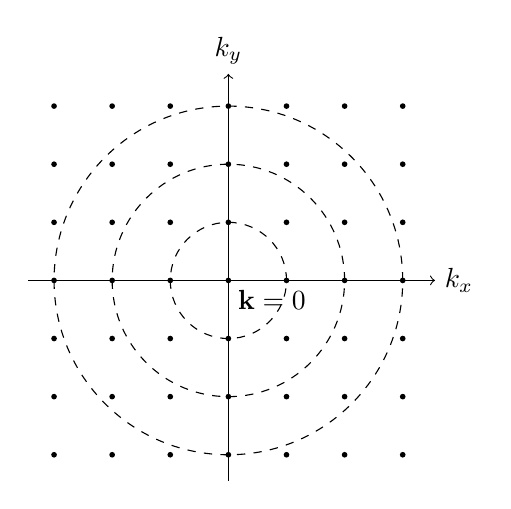
\begin{tikzpicture}[scale=0.82]
\draw[->] (-3.1,0) -- (3.2,0) node[right] {$k_x$};
\draw[->] (0,-3.1) -- (0,3.2) node[above] {$k_y$};
\draw[dashed] (0,0) circle (0.9);
\draw[dashed] (0,0) circle (1.8);
\draw[dashed] (0,0) circle (2.7);
\foreach \x in {-3,-2,-1,0,1,2,3}{
  \foreach \y in {-3,-2,-1,0,1,2,3}{
    \fill (0.9*\x,0.9*\y) circle (1.25pt);
  }
}
\node[below right] at (0,0) {$\mathbf{k}=0$};
\end{tikzpicture}
\caption{Các trạng thái xung lượng rời rạc và các lớp năng lượng không đổi của các hạt trong một hộp hữu hạn với điều kiện biên tuần hoàn.}
\end{figure}

Đối với một hạt không tương đối tính,
\begin{equation}
E_{\mathbf{k}}=\frac{\mathbf{k}^2}{2m},
\end{equation}
nên trạng thái có năng lượng thấp nhất là \(\mathbf{k}=0\). Đặt \(N\) boson đồng nhất vào hộp và tìm trạng thái cơ bản nhiều hạt. Boson thứ nhất đi vào trạng thái xung lượng bằng không. Boson thứ hai có thể đi vào cùng trạng thái đó, cũng như boson thứ ba và mọi boson tiếp theo. Vì vậy, cả \(N\) boson đều chiếm \(\mathbf{k}=0\).

Đây là một ngưng tụ boson: một số lớn hạt đồng nhất cùng chiếm một trạng thái một hạt, ở đây là trạng thái năng lượng thấp nhất. Hàm sóng xung lượng bằng không là hằng theo không gian và trải khắp hộp. Nó không định xứ bất kỳ boson nào tại một vị trí cụ thể; vì thế mỗi boson đều bất định về việc nó ở đâu. Khi số chiếm đóng trở nên lớn, hàm sóng chung tích lũy thành một biên độ trường vĩ mô, và trường ngày càng ứng xử giống một trường cổ điển.

Trạng thái cơ bản fermion hoàn toàn khác. Tạm thời bỏ qua spin, để mỗi điểm xung lượng biểu diễn một trạng thái khả dụng. Fermion thứ nhất đi vào \(\mathbf{k}=0\), nhưng một fermion đồng nhất thứ hai không thể vào cùng nó. Các hạt tiếp theo phải chiếm lớp năng lượng thấp kế tiếp. Trong một hình vẽ hai chiều có bốn điểm mạng khác không gần nhất có cùng năng lượng; trong ba chiều có sáu điểm. Sau khi các trạng thái đó bị chiếm, những hạt tiếp theo phải đi vào các lớp kế tiếp.

Bởi vì năng lượng tỉ lệ với bình phương khoảng cách đến gốc trong không gian xung lượng, việc tối thiểu hóa tổng năng lượng có nghĩa là sắp các điểm bị chiếm sít nhất có thể quanh \(\mathbf{k}=0\), trong giới hạn nguyên lý loại trừ cho phép. Với nhiều fermion, vùng bị chiếm xấp xỉ một khối cầu. Biên của nó là bề mặt Fermi, phần bên trong là biển Fermi, và toàn bộ vùng được lấp đầy là khối cầu Fermi. Ở thể tích hữu hạn, biên hơi lởm chởm vì các điểm khả dụng tạo thành một mạng, nhưng chi tiết này trở nên không đáng kể đối với một hệ lớn.

\begin{figure}
\centering
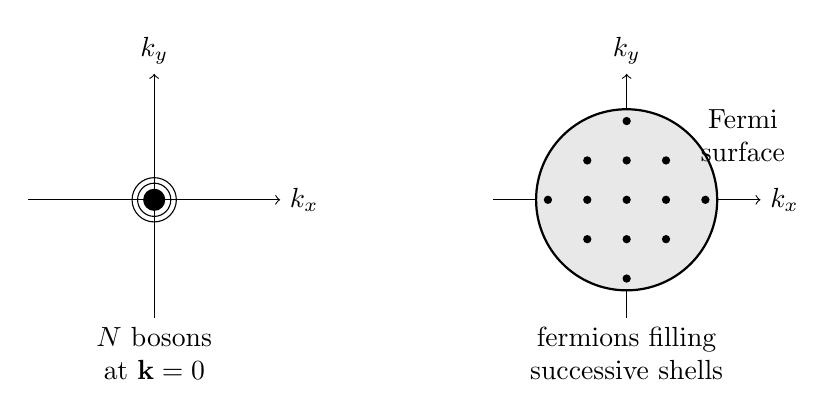
\begin{tikzpicture}[scale=1.0]
\begin{scope}[xshift=-3.0cm]
\draw[->] (-1.6,0) -- (1.6,0) node[right] {$k_x$};
\draw[->] (0,-1.5) -- (0,1.6) node[above] {$k_y$};
\fill (0,0) circle (4pt);
\draw (0,0) circle (6pt);
\draw (0,0) circle (8pt);
\node[align=center] at (0,-1.95) {$N$ bosons\\at $\mathbf{k}=0$};
\end{scope}
\begin{scope}[xshift=3.0cm]
\draw[->] (-1.7,0) -- (1.7,0) node[right] {$k_x$};
\draw[->] (0,-1.5) -- (0,1.6) node[above] {$k_y$};
\fill[gray!18] (0,0) circle (1.15);
\draw[thick] (0,0) circle (1.15);
\fill (0,0) circle (1.5pt);
\fill (0.5,0) circle (1.5pt);
\fill (-0.5,0) circle (1.5pt);
\fill (0,0.5) circle (1.5pt);
\fill (0,-0.5) circle (1.5pt);
\fill (0.5,0.5) circle (1.5pt);
\fill (0.5,-0.5) circle (1.5pt);
\fill (-0.5,0.5) circle (1.5pt);
\fill (-0.5,-0.5) circle (1.5pt);
\fill (1,0) circle (1.5pt);
\fill (-1,0) circle (1.5pt);
\fill (0,1) circle (1.5pt);
\fill (0,-1) circle (1.5pt);
\node[right,align=center] at (0.82,0.82) {Fermi\\surface};
\node[align=center] at (0,-1.95) {fermions filling\\successive shells};
\end{scope}
\end{tikzpicture}
\caption{Boson ngưng tụ vào trạng thái có xung lượng bằng không, còn fermion lấp đầy các trạng thái xung lượng từ trong ra ngoài cho tới một bề mặt Fermi.}
\end{figure}

Trạng thái cơ bản fermion có năng lượng lớn hơn rất nhiều so với trạng thái cơ bản boson tương ứng. Tất cả boson đều có thể ở lại tại xung lượng bằng không, nhưng phần lớn fermion buộc phải ở các trạng thái xung lượng khác không. Khi thêm nhiều fermion hơn, xung lượng bị chiếm lớn nhất tăng lên. Hơn nữa, một lớp ở xung lượng lớn chứa nhiều điểm mạng hơn một lớp gần gốc. Vì vậy, một khối cầu Fermi lớn chứa nhiều hạt có xung lượng đáng kể và chỉ một số nhỏ trong các trạng thái xung lượng thấp nhất.

Sự tương phản còn tiếp tục ở các trạng thái kích thích. Đối với boson, kích thích đầu tiên thu được bằng cách lấy một boson bất kỳ ra khỏi trạng thái ngưng tụ và đặt nó vào trạng thái một hạt kích thích thứ nhất:
\begin{equation}
(N,0,0,\ldots)\longrightarrow (N-1,1,0,\ldots).
\end{equation}
Không quan trọng boson nào bị chuyển; các hạt là đồng nhất. Có thể tạo các kích thích cao hơn theo vài cách. Tùy vào khoảng cách mức năng lượng, ta có thể đặt một boson vào một mức cao hơn hoặc đặt hai boson vào mức kích thích thứ nhất. Kích thích hệ boson có nghĩa là nâng các hạt ra khỏi trạng thái ngưng tụ lên các trạng thái năng lượng cao hơn.

Đối với fermion, không hạt nào có thể được chuyển tới một điểm khác bên trong khối cầu Fermi đã lấp đầy, vì mọi điểm như vậy đều đã bị chiếm. Lấy một fermion từ sâu trong biển và đặt nó lên trên bề mặt là điều có thể, nhưng tốn một năng lượng lớn. Kích thích ít tốn kém nhất lấy một fermion từ ngay bên trong bề mặt Fermi và chuyển nó tới một trạng thái chưa bị chiếm ngay bên ngoài. Electron được nâng lên chỉ có năng lượng cao hơn bề mặt một lượng nhỏ, và trạng thái trống còn lại chỉ thấp hơn bề mặt một lượng nhỏ.

\begin{figure}
\centering
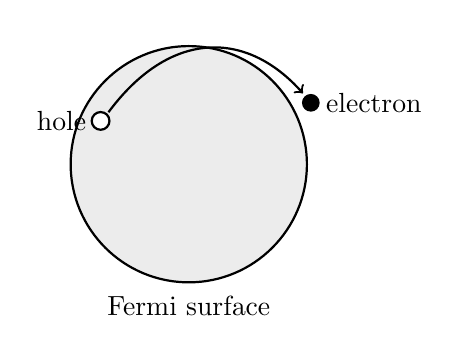
\begin{tikzpicture}[scale=1.0]
\fill[gray!15] (0,0) circle (1.5);
\draw[thick] (0,0) circle (1.5);
\draw[fill=white,thick] (-1.12,0.55) circle (3.2pt);
\fill (1.55,0.78) circle (3.2pt);
\draw[->,thick] (-1.02,0.66) .. controls (-0.25,1.7) and (0.72,1.72) .. (1.45,0.9);
\node[left] at (-1.18,0.55) {hole};
\node[right] at (1.62,0.78) {electron};
\node[below] at (0,-1.55) {Fermi surface};
\end{tikzpicture}
\caption{Một kích thích fermion năng lượng thấp đưa một electron xuyên qua bề mặt Fermi và để lại một lỗ trống phía sau.}
\end{figure}

\section{Lỗ trống và các kích thích năng lượng thấp}

Để làm rõ điện tích của lỗ trống, hãy hình dung hộp chứa điện tích dương được trải đều khắp thể tích của nó. Trong vật chất, điện tích dương đó rốt cuộc đến từ các proton trong hạt nhân, nhưng phân bố đều giữ cho mô hình đơn giản. Hãy thêm đủ electron để trung hòa nền điện tích ấy. Ở trạng thái cơ bản, các electron đó lấp đầy khối cầu Fermi.

Nâng một electron từ dưới lên trên bề mặt Fermi không làm thay đổi tổng điện tích của hộp. Việc đó tạo ra một electron mang điện âm ở phía trên bề mặt và để lại bên dưới nó một phần điện tích âm bị thiếu. Vì thế electron bị thiếu có thể được xem như một kích thích mang điện dương: một lỗ trống.

\begin{classroomqa}
\lecturetimestamp{01:31:38}
\audiencequestion{Liệu một lỗ trống ở dưới bề mặt Fermi có năng lượng âm hay không?}
\lecturerresponse{Không. Lỗ trống là một kích thích ở trên trạng thái cơ bản nhiều hạt, nên năng lượng kích thích của nó là dương. Việc lấy một electron đang bị chiếm ra khỏi phía dưới bề mặt Fermi tốn một lượng năng lượng dương khi năng lượng được đo so với bề mặt ấy.}
\end{classroomqa}

Gọi electron bị lấy đi có năng lượng \(\varepsilon<\varepsilon_F\), và electron được nâng lên có năng lượng \(\varepsilon'>\varepsilon_F\). Năng lượng được cung cấp có thể được tách thành hai độ lệch dương khỏi bề mặt Fermi.\footnote{Hai khoảng này được nêu riêng rẽ; đẳng thức gọn được hiển thị ở đây là cách viết lại tương đương về mặt đại số.}
\begin{equation}
\Delta E
=\varepsilon'-\varepsilon
=(\varepsilon'-\varepsilon_F)+(\varepsilon_F-\varepsilon).
\end{equation}
Phần đóng góp thứ nhất được gán một cách tự nhiên cho electron ở trên bề mặt Fermi, còn phần thứ hai được gán cho lỗ trống ở dưới nó:
\begin{equation}
E_{\mathrm{electron}}=\varepsilon'-\varepsilon_F>0,
\qquad
E_{\mathrm{hole}}=\varepsilon_F-\varepsilon>0.
\end{equation}
Electron mang điện tích âm, còn lỗ trống mang điện tích dương.

Một electron ở trên bề mặt Fermi về sau có thể rơi vào một lỗ trống khả dụng. Khi đó năng lượng của nó giảm, nên bức xạ phải mang năng lượng được giải phóng đi. Có thể mô tả sự kiện này như một electron rơi xuống một trạng thái thấp hơn chưa bị chiếm và phát ra một hay nhiều photon. Tương đương, ta có thể nói rằng một electron và một lỗ trống hủy nhau thành bức xạ. Lỗ trống không phải là một thành phần cơ bản bổ sung của cái hộp; nó là sự vắng mặt trong trạng thái nhiều electron đã lấp đầy. Tuy nhiên, năng lượng và điện tích của nó khiến việc xem nó như một kích thích kiểu hạt trở nên hữu ích.

\begin{classroomqa}
\lecturetimestamp{01:36:52}
\audiencequestion{Việc nâng một electron có nghĩa là chuyển nó từ điểm mạng này sang điểm mạng khác trong không gian xung lượng hay không?}
\lecturerresponse{Nó có nghĩa là chuyển electron từ mức năng lượng này sang mức năng lượng khác. Đối với các hạt tự do trong hộp, mạng xung lượng gắn nhãn các mức đó, nhưng ý tưởng ấy không phụ thuộc vào một mạng trong không gian xung lượng. Trong nguyên tử, điện tích dương tập trung ở hạt nhân. Các electron lấp đầy các mức nguyên tử khả dụng thấp nhất, và một photon có thể nâng một electron lên một mức kích thích, để lại một chỗ trống ở mức mà nó xuất phát. Chỗ trống đó là đối ứng trong nguyên tử của một lỗ trống.}
\end{classroomqa}

Trong hộp, sự hấp thụ photon tương tự cũng chuyển năng lượng photon thành một electron ở trên bề mặt Fermi và một lỗ trống ở dưới nó. Trong nguyên tử, cùng ngôn ngữ ấy mô tả electron bị kích thích cùng với chỗ trống còn lại trong các mức thấp hơn đang bị chiếm.

\begin{classroomqa}
\lecturetimestamp{01:39:16}
\audiencequestion{Liệu một photon năng lượng thấp có thể được một electron hấp thụ ở bất cứ đâu trong khối cầu Fermi hay không?}
\lecturerresponse{Không. Nếu electron nằm sâu trong biển Fermi, thì mọi trạng thái lân cận đều đã bị chiếm, và một photon năng lượng thấp không thể nâng nó lên tận một trạng thái chưa bị chiếm ở phía trên bề mặt. Chỉ những electron đủ gần bề mặt Fermi mới có các trạng thái trống khả dụng trong miền năng lượng của photon. Một photon đủ năng lượng có thể kích thích một electron từ sâu trong biển.}
\end{classroomqa}

Vì vậy, tiết diện hấp thụ năng lượng thấp được quyết định bởi bề mặt của biển Fermi chứ không phải bởi toàn bộ thể tích của nó. Các electron sâu trong biển bị chặn không thể thực hiện những chuyển dời nhỏ; các electron ngay dưới bề mặt có thể được chuyển lên ngay trên nó.

\begin{classroomqa}
\lecturetimestamp{01:40:42}
\audiencequestion{Điều gì ngăn electron tương tác trực tiếp với nhau, mà không cần một photon tới?}
\lecturerresponse{Không có gì cả. Các tương tác electron--electron bị bỏ qua trong mô hình đơn giản này, vì đưa chúng vào sẽ làm bức tranh biển Fermi phức tạp hơn. Trong phép gần đúng đầu tiên này cho một kim loại, ảnh hưởng hiệu dụng của chúng được xem là đủ yếu để thường có thể bỏ qua.}
\end{classroomqa}

\begin{classroomqa}
\lecturetimestamp{01:41:10}
\audiencequestion{Điều gì xảy ra nếu một photon mang đủ năng lượng để kích thích vài electron?}
\lecturerresponse{Về nguyên tắc, mọi quá trình phù hợp với các định luật bảo toàn đều có thể xảy ra. Photon có thể tạo ra nhiều hơn một cặp electron--lỗ trống: kích thích hai electron cũng để lại hai lỗ trống. Một quá trình như vậy tạo ra nhiều kích thích hơn và nhìn chung có xác suất nhỏ hơn so với việc dùng năng lượng đó để kích thích một electron mạnh hơn nhiều.}
\end{classroomqa}

\begin{classroomqa}
\lecturetimestamp{01:42:06}
\audiencequestion{Hai photon có thể được hấp thụ đồng thời khi bản thân từng photon riêng lẻ đều không thể tạo ra kích thích đó không?}
\lecturerresponse{Có. Sự hấp thụ mang tính xác suất, và một quá trình hai photon có thể xảy ra khi tổng năng lượng của hai photon đạt tới một mức kích thích khả dĩ, mặc dù từng photon riêng lẻ đều thấp hơn năng lượng cần thiết. Nếu ánh sáng sẵn có mang năng lượng quá nhỏ để đạt tới bất kỳ kích thích được phép nào, thì phần lớn nó sẽ truyền qua hệ.}
\end{classroomqa}

\editorialnote{Một thảo luận ngắn ở chỗ này liên hệ bức xạ bị hấp thụ với chuyển động tập thể của electron, nhưng các chi tiết nội dung của nó không thể khôi phục được. Chỉ có nhận định rằng đáp ứng tập thể như vậy phức tạp hơn bức tranh hạt--lỗ trống đơn là chắc chắn.}

\begin{classroomqa}
\lecturetimestamp{01:43:49}
\audiencequestion{Tại sao các tương tác electron--electron được gọi là yếu khi mọi electron đều mang cùng một điện tích âm?}
\lecturerresponse{Các electron được nhúng trong một nền dương bù trừ. Nền đó che chắn điện tích của một electron và làm giảm tương tác hiệu dụng trong bối cảnh đơn giản hóa này. Tương tác không phải là không có; việc xử lý nó đòi hỏi đáp ứng che chắn của môi trường.}
\end{classroomqa}

\begin{classroomqa}
\lecturetimestamp{01:44:41}
\audiencequestion{Hiệu ứng che chắn sẽ được thảo luận sau chứ?}
\lecturerresponse{Có. Hiệu ứng che chắn là quan trọng, nhưng được để lại cho đến khi hệ tương tác có thể được xử lý đầy đủ hơn.}
\end{classroomqa}

\section{Biển fermion một chiều và phản hạt}

Cách xây dựng lỗ trống gợi đến phản hạt. Cùng một cấu trúc logic đó có thể được chuyển từ các electron trong vật chất sang một trường lượng tử tương đối tính và chân không của nó. Phiên bản đơn giản nhất dùng một chiều không gian và một trường fermion không khối lượng \(\psi(x,t)\). Trong hệ đơn vị mà tốc độ ánh sáng bằng một, hai quan hệ tán sắc tuyến tính khả dĩ là
\begin{equation}
\omega=k,
\qquad\text{or}\qquad
\omega=-k.
\end{equation}
Nhánh thứ nhất sẽ được xét tường minh.

\editorialnote{Phần trao đổi cuối cùng luân phiên giữa các cách đồng nhất hạt không tương thích với nhau. Mô hình có thể xác định chắc chắn là một trường fermion đồ chơi không khối lượng, không được chỉ rõ, trong một chiều không gian, bị giới hạn ở một hướng lan truyền.}

Đối với một sóng phẳng
\begin{equation}
\psi(x,t)=e^{i(kx-\omega t)},
\end{equation}
các đạo hàm là
\begin{equation}
\frac{\partial\psi}{\partial t}=-i\omega\psi,
\qquad
\frac{\partial\psi}{\partial x}=ik\psi.
\end{equation}
Vì vậy, \(\omega=k\) tương đương với phương trình trường bậc nhất
\begin{equation}
\frac{\partial\psi}{\partial t}
=-\frac{\partial\psi}{\partial x}.
\end{equation}

\begin{figure}
\centering
\includegraphics[width=0.72\textwidth]{lecture_05_figure_05.png}
\caption{Khởi đầu từ phương trình trường bậc nhất mà các sóng phẳng của nó thỏa mãn \(\omega=k\).}
\lectureframe{01:47:22}
\end{figure}

Mọi biên dạng có dạng \(f(x-t)\) đều thỏa mãn phương trình này và truyền sang phải. Đảo dấu cho
\begin{equation}
\frac{\partial\psi}{\partial t}
=+\frac{\partial\psi}{\partial x},
\end{equation}
mà các biên dạng \(f(x+t)\) của nó truyền sang trái. Mỗi phương trình bậc nhất chỉ chọn ra một hướng chuyển động. Hãy giả sử đây là một trường fermion và, để lập luận về lỗ trống, giả sử rằng các hạt của nó mang điện tích.

Nhánh \(\omega=k\) chứa một khó khăn xuất hiện ngay lập tức. Số sóng \(k\) có thể âm, và vì thế \(\omega\) cũng có thể âm. Vì \(\omega\) là năng lượng trong hệ đơn vị này, phổ đường thẳng ấy chứa cả các trạng thái năng lượng dương lẫn năng lượng âm:
\begin{equation}
E=\omega=k.
\end{equation}

\begin{figure}
\centering
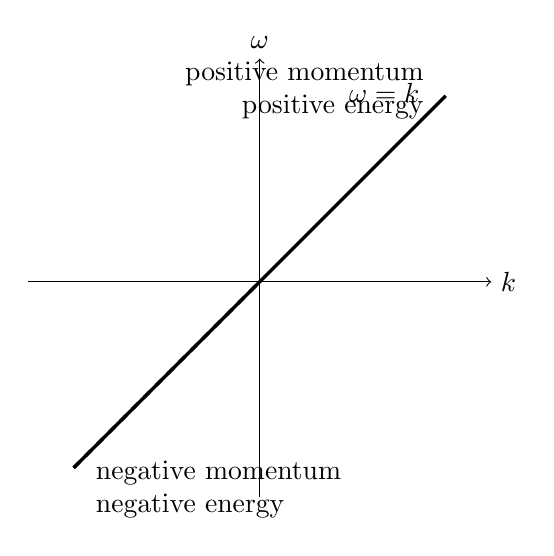
\begin{tikzpicture}[scale=1.05]
\draw[->] (-2.8,0) -- (2.8,0) node[right] {$k$};
\draw[->] (0,-2.6) -- (0,2.7) node[above] {$\omega$};
\draw[very thick] (-2.25,-2.25) -- (2.25,2.25);
\draw[very thick,dashed] (-2.25,-2.25) -- (0,0);
\node[above left] at (2.05,2.05) {$\omega=k$};
\node[below right,align=left] at (-2.1,-2.05) {negative momentum\\negative energy};
\node[above left,align=right] at (2.1,1.85) {positive momentum\\positive energy};
\end{tikzpicture}
\caption{Phổ một nhánh \(\omega=k\), với một nửa mang năng lượng âm nằm ở \(k<0\).}
\end{figure}

Một chân không rỗng thông thường không thể là trạng thái cơ bản của một lý thuyết như vậy. Một fermion năng lượng dương có thể bức xạ ra một photon và rơi xuống một trạng thái thấp hơn. Không có gì buộc nó phải dừng ở 0: nó có thể tiếp tục đi vào các trạng thái năng lượng âm, phát ra thêm bức xạ nữa và rơi xuống không bị chặn. Năng lượng mà fermion mất đi sẽ xuất hiện trong trường bức xạ. Vì vậy, một phổ không bị chặn dưới không cho một chân không thông thường ổn định.

Nguyên lý loại trừ fermion cung cấp một điểm xuất phát khác. Hãy lấp đầy mỗi trạng thái một hạt có năng lượng âm, tới năng lượng 0, bằng một fermion. Không fermion nào khác có thể rơi vào những trạng thái đó vì mỗi trạng thái đều đã bị chiếm. Việc thêm một fermion năng lượng âm khác là không thể, trong khi thêm một fermion năng lượng dương thì làm tăng năng lượng. Vì thế, biển năng lượng âm được lấp đầy hoàn toàn có thể được coi là trạng thái cơ bản nhiều hạt và được gọi là chân không.

\begin{figure}
\centering
\resizebox{\linewidth}{!}{%
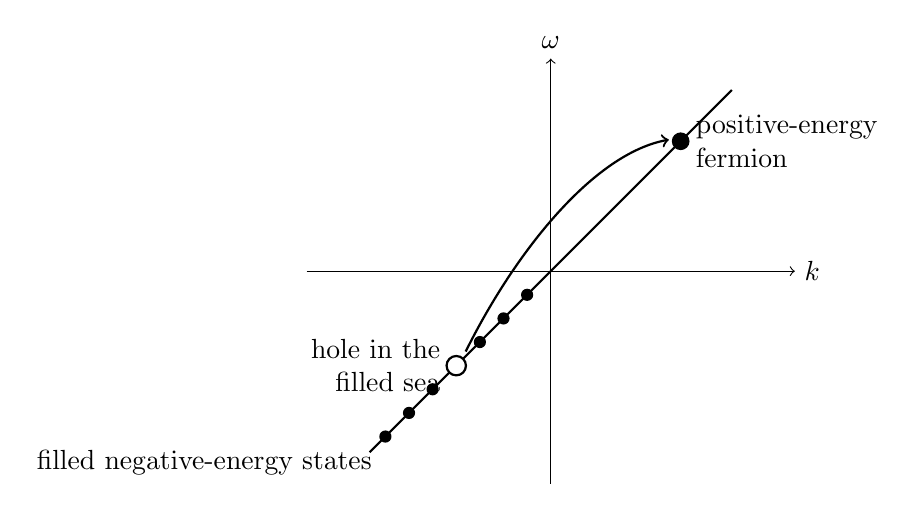
\begin{tikzpicture}[scale=1.0]
\draw[->] (-3.1,0) -- (3.1,0) node[right] {$k$};
\draw[->] (0,-2.7) -- (0,2.7) node[above] {$\omega$};
\draw[thick] (-2.3,-2.3) -- (2.3,2.3);
\foreach \p in {-2.1,-1.8,-1.5,-1.2,-0.9,-0.6,-0.3}{
  \fill (\p,\p) circle (2.2pt);
}
\draw[fill=white,thick] (-1.2,-1.2) circle (3.5pt);
\fill (1.65,1.65) circle (3.2pt);
\draw[->,thick] (-1.08,-1.02) .. controls (-0.45,0.25) and (0.55,1.5) .. (1.5,1.67);
\node[left,align=right] at (-1.28,-1.2) {hole in the\\filled sea};
\node[right,align=left] at (1.72,1.65) {positive-energy\\fermion};
\node[below left] at (-2.15,-2.15) {filled negative-energy states};
\end{tikzpicture}%
}
\caption{Biển năng lượng âm đã lấp đầy và một kích thích được tạo ra bằng cách nâng một fermion lên năng lượng dương.}
\end{figure}

Kích thích đơn giản nhất lấy một fermion ra khỏi biển năng lượng âm và đặt nó vào một trạng thái năng lượng dương. Fermion được nâng lên là một hạt năng lượng dương thông thường. Chỗ khuyết để lại trong biển là một kích thích thứ hai, một lỗ trống. Nếu fermion bị lấy đi mang điện tích âm, thì lỗ trống mang điện tích dương.

Lỗ trống cũng có xung lượng dương trong ví dụ một nhánh này. Nếu fermion bị thiếu đã chiếm một trạng thái có xung lượng \(k_-<0\), thì việc lấy nó đi làm thay đổi tổng xung lượng một lượng
\begin{equation}
p_{\mathrm{hole}}=-k_->0.
\end{equation}
Đó là sự thiếu hụt của xung lượng âm. Vì thế, kích thích này gồm một fermion năng lượng dương mang điện tích âm và một lỗ trống năng lượng dương mang điện tích dương. Cả hai đều mang xung lượng dương và, trên nhánh \(\omega=k\), cả hai đều chuyển động sang phải.

Trong lý thuyết đầy đủ về electron, lỗ trống mang điện tích dương là positron. Ban đầu Dirac từng cân nhắc việc đồng nhất lỗ trống với proton. Cách xây dựng này đòi hỏi một hạt và phản hạt của nó phải có cùng khối lượng. Lỗ trống là một hạt riêng biệt, có khối lượng của electron và điện tích đối dấu. Đây là cách diễn giải hạt--phản hạt cơ bản mà phổ năng lượng âm đã dẫn tới.

Không thể áp dụng cùng cách cứu vãn đó cho boson. Một trạng thái boson cho phép số hạt tùy ý, nên không có cách nào lấp đầy một mức năng lượng âm một lần rồi ngăn sự chiếm thêm. Luôn luôn có thể thêm nhiều boson hơn vào mức đó, làm hạ năng lượng hết lần này đến lần khác:
\begin{equation}
\begin{aligned}
\text{fermionic mode: }&n=0\ \text{or}\ 1,\\
\text{bosonic mode: }&n=0,1,2,\ldots .
\end{aligned}
\end{equation}
Hệ boson được đề xuất khi đó vẫn sẽ không có trạng thái cơ bản. Trong cách xây dựng sơ cấp này, tính ổn định của biển đã lấp đầy phụ thuộc chính xác vào nguyên lý loại trừ fermion.

Phương trình một chiều này chỉ là một phiên bản đồ chơi của phương trình Dirac. Trường của nó không khối lượng, chuyển động với tốc độ ánh sáng và chỉ lan truyền theo một hướng. Một phương trình Dirac đầy đủ hơn phải bao hàm các hướng chuyển động còn thiếu và phần còn lại của cấu trúc hạt tương đối tính. Phương trình đầy đủ hơn đó, cùng với việc xử lý phản hạt đối với các trường boson, được để lại cho sau.